
\documentclass{beamer}
\usepackage{graphicx}
\usepackage{verbatim}
\usepackage{listings-lua}
\usepackage{tikz}


\mode<presentation> {
\usetheme{Madrid}
%\usecolortheme{default}
%\setbeamertemplate{navigation symbols}{} 
}

% TikZ setup:
\usetikzlibrary{arrows,shapes,positioning,shadows,trees}
\begin{document}

\title[GRR, ARGH]{Generic Resource Representation,\\
                  Abstract Resource Grouping Hierarchy \\
                  (GRR, ARGH)}
\subtitle{Concepts for a Flux Resource Inventory.}
\author[Grondona]{Mark A. Grondona}
\institute{LLNL}
\date{\today}


% Title slide:
\maketitle

\begin{frame}{Resource Inventory High Level Requirements}
\begin{itemize}
 \item {\em Dynamic} data store for Flux resources
 \item Sitewide service for resource discovery and tracking 
 \begin{itemize}
        \item Example: replace static ``cluster info'' pages
 \end{itemize}
 \item Store arbitrary relationships between resources
 \item Common interface for Flux, user, and middleware tools to communicate
        about resources
 \item Extensible: good tools for extending existing resource types
 \item Hierarchical\ldots
 \item {\em but}, also able to express arbitrary topology between resources
 \item Subset of a RI must also be a valid RI \\
       (support hierarchical job model)
 \item Generalized -- no dependency on preconceptions
 \item Dynamic: support {\em grow}/{\em shrink}
 \item Simple language interface for easy configuration
\end{itemize}
\end{frame}

\begin{frame}{Resource Inventory}{Conceptual Discussion}
\vskip 1em
{\em At least} 3 components in even minimal working Resource Inventory:
\vskip 1em
\begin{enumerate}
 \item Backend DB or storage
 \item \alert<2-> {Resource description and/or configuration language}
 \item \alert<3-> {API to query/update resources}
\end{enumerate}
\end{frame}

\begin{frame}{Resource Description Language}{Topics}
\begin{itemize}
 \item High level concept: {\em composite resources}
 \item Resource ``classes''
 \item Resource instances
 \item Conceptual language syntax
\end{itemize}
\end{frame}

\begin{frame}{Resource Language Abstraction}{The Composite Resource}
\begin{definition}
A {\em composite resource} is a resource which is composed of other
resources, each of which may also be a composite.
\end{definition}
\vskip 1em
Examples: ComputeNode is a composite of Memory and Sockets, and Socket is
a composite of cores and threads, \ldots

Useful properties of a composite
\begin{itemize}
 \item Individual resources and collections of resources have the same
       interface (supports subset of inventory is also a valid inventory)
 \item Naturally hierarchical
 \item Promote resource {\em class} reuse
 \item Well understood/researched programming pattern
\end{itemize}
\end{frame}

\begin{frame}{Composite Resource Model}{Risks}
\vskip 1em
Even if composite resource is a useful concept, we may not want to be
formal or pedantic about it, as there are some risks:
\vskip 1em
\begin{itemize}
 \item Can the abstraction support resource types like power and bandwidth?
 \item Artificially confining or limiting?
 \item Introduces more complexity than it is worth
\end{itemize}
\end{frame}

\begin{frame}{Composite Resource Implementation}{``Class'' Attributes}
\begin{itemize}
 \item Constructor with variable args (e.g. as table of key/values)
 \item Class-static properties
 \item Operations (e.g {\tt contain()})
 \item Relations (parent)
 \item Associations (e.g. {\em myNode has 2 HaswellSockets})
 \item Base methods include ability to set a tag on a resource and
    getter/setters for other variables
\end{itemize}
\end{frame}

\begin{frame}{Composite Resource Implementation, continued\ldots}
{\centering Resource ``Instance'' Attributes:}
\begin{description}
 \item[ID] Local id within a parent or ancestor (e.g. $0$ or maybe socket$0$)
 \item[Name] For named resources, e.g. a hostname, logical cpuid
 \item[uri]  Full path to this instance in a ``master'' heirarchy \\
             e.g. {\tt gov.llnl.hype.switch0.node1 }
 \item[attributes] e.g. label=, vendor=, ...
 \item[tags] allocated, drained, \ldots
 \item[topologies] Pointers into layouts or topologies in which this resource
                    belongs
 \item[children] List of components within this resource
 \item[parent]   Pointer to component in which this instance is a member
\end{description}
\end{frame}

\begin{frame}[fragile]{Composite Resource Implementation, continued\ldots}
\centering
\begin{tikzpicture}
\node [fill=purple!32!blue!12,
       rectangle,
       rounded corners=5pt,
       draw, thick, drop shadow] (code) {%
\begin{minipage}[b][15em][c]{.95\textwidth}
\vskip 1em
\begin{lstlisting}[%
  language={[5.1]Lua},%
  basicstyle=\footnotesize\ttfamily,%
  keywordstyle=\footnotesize\color{blue}\ttfamily,%
  stringstyle=\footnotesize\color{green!98}\ttfamily,%
  commentstyle=\itshape\color{red!20!black}\ttfamily,% comments
  rulesepcolor=\color{black},%
]
mySocket = {
  parent = Socket,
  constructor = function (args) 
     local self = Socket.new (args)
     self:add_attributes{ vendor = "foo", model = "bar" }
     for i in 1,arg.ncores do
         core = myCore.new{ myattr = "value" }
         self.add_child (core)
     end
     return self
  end,
}
\end{lstlisting}
\end{minipage}
};
\node [fill=blue!28, rectangle, rounded corners, draw, thick] at (code.north) {%
config syntax mockup
};
\end{tikzpicture}
\end{frame}

\begin{frame}{Composite Resource Concepts}{Aggregation and Delegation}
\vskip 1em
Composite model also lends itself to some high-level operations that
more directly support Flux components and users
\vskip 1em
\begin{itemize}
 \item {\em aggregation}: summarizes information from components up the tree \\
  {\centering {\tt Cluster = \{ nodes = 1024, cores = 16384, ...\}}}
  \vskip 1em
 \item {\em delegation}: delegates methods and queries up the tree
 \begin{itemize}
  \item e.g. lookup of a {\em hostname} attribute for a CPU delegates to parent
       object (a {\em Socket}) which delegates to its parent (a {\em Node})
 \end{itemize}
\end{itemize}
\end{frame}

\begin{frame}{Composite Resource Concepts}{Parent Delegation}
\begin{itemize}
 \item<+-> Some attributes local to parent ``resources'' may need to be accessed
       from children.
 \visible<+->{\begin{itemize}
   \item e.g. imagine a job running on a single CPU/processing unit
   \item ``Inventory'' for this job should have the same interface as
          an inventory encompassing a whole node, or even an entire cluster.
   \item How do we handle request for ``what is your address?''
 \end{itemize}}
 \visible<3->{\item Therefore, children may need to delegate some methods or
             attribute queries to a parent}
 \visible<4->{\item e.g. Address query on a {\em CPU} delegates the request
              to {\em Socket}, which delegates to {\em Node}}
\end{itemize}
\end{frame}

\begin{frame}{Composite Resource Concepts}{Aggregation}
\begin{itemize}
\item Essentially a summary query on a composite resource
       "What do you contain?"
\item Natural to implement this as tree reduction
\item Many modern DBs support applicable map/reduce functionality
\end{itemize}
\end{frame}


\begin{frame}{Composite Resource Tags}
\visible<+->{%
Use of {\em tags} on resources as a general feature a key point in
our vision paper.
}
\vskip 1em
\visible<+->{Possible {\em tagging} operations:}
\begin{itemize}
 \item<+-> {\em add TAG}: Add TAG to current resource
 \item<+-> {\em remove TAG}: Remove a tag
 \item<+-> {\em recursive-\{add,remove\} TAG}: Add/remove tag from children
 \item<+-> {\em search TAG}: Return list of resources with TAG
 \item<+-> {\em inclusive-search TAG}: Return all resources with tag,
	     including children
 \item<+-> {\em prune TAG}: Prune resources from current composite at TAG
\end{itemize}
\end{frame}

%\begin{frame}{Queries and Resource Specification}
%Requirements
%\begin{itemize}
% \item Flexibile -- resource specification syntax should grow
%       and adapt with Flux
% \item Powerful -- better than existing software which supports targetting
%       nodes, sockets, cores, threads, etc.
% \item Extensible -- Allow users and administrators to extend the
%       language with site-local enhancements
%\end{itemize}
%\end{frame}

\begin{frame}[fragile]{Example: Matching Composite Resources}
  \begin{tikzpicture}[
    every node/.style = {drop shadow, rectangle, rounded corners,
        fill=blue!25, draw, thick},
    level 1/.style = {sibling distance = 6cm},
    level 3/.style = {sibling distance = 2.5cm},
    level 4/.style = {sibling distance = 12mm, font=\tiny},
    level 5/.style = {sibling distance = 7mm, font=\tiny, circle},
    level distance = 10mm,
    text depth = 0pt
   ]
    \hspace{-2mm}% Arggh, is there a better way to remove left margin?
    \node (center) {center}
      child {node (clusterA) {cluster A}
        child {node (switch0) {switch 0}
          child {node (n0) {n0}
            child {node (n0S0) {S0}
              child {node (n0S0cpu0) {cpu0}}
              child {node (n0S0cpu1) {cpu1}}
            }
            child {node (n0S1) {S1}
              child {node (n0S1cpu0) {cpu0}}
              child {node (n0S1cpu1) {cpu1}}
            }
          }
          child {node (n1) {n1}
            child {node (n1S0) {S0}
              child {node (n1S0cpu0) {cpu0}}
              child {node (n1S0cpu1) {cpu1}}
            }
            child {node {S1}
              child {node {cpu0}}
              child {node {cpu1}}
            }
          }
          child {node {n2}
            child {node {S0}
              child {node {cpu0}}
              child {node {cpu1}}
            }
            child {node {S1}
              child {node {cpu0}}
              child {node {cpu1}}
            }
          }
        }
%
%
        child {node {switch 1}
          child {node {n3}
            child {node {S0}
              child {node {cpu0}}
              child {node {cpu1}}
            }
            child {node {S1}
              child {node {cpu0}}
              child {node {cpu1}}
            }
          }
          child {node {n4}
            child {node {S0}
              child {node {cpu0}}
              child {node {cpu1}}
            }
            child {node {S1}
              child {node {cpu0}}
              child {node {cpu1}}
            }
          }
        }
      } ;

    \visible<2->{\node [fill=green!32] (request) at (3,.5) {%
      \begin{minipage}[b][6em][c]{.33\linewidth}
 	\[% 
         \delimiterfactor=1500
         \left\{%
         \begin{array}{ll}
           nodes &== 2, \\ cpus &== 6.
         \end{array}%
         \right\}%
         \]
      \end{minipage}
     }; 
     \node [fill=blue!48] at (request.north) {request};
    }

    \only<3->{\node [fill=red!64] at (center) {center}};
    \only<4->{\node [fill=red!64,] at (clusterA) {cluster A}};
    \only<5->{\node [fill=red!64] at (switch0) {switch 0}};
    \only<6->{\node [fill=red!64] at (n0) {n0}};
    \only<7->{\node [fill=red!64] at (n0S0) {\tiny S0}; 
              \node [fill=red!64] at (n0S1) {\tiny S1};
              \node [fill=red!64] at (n0S0cpu0) {\tiny cpu0};
              \node [fill=red!64] at (n0S0cpu1) {\tiny cpu1};
              \node [fill=red!64] at (n0S1cpu0) {\tiny cpu0};
              \node [fill=red!64] at (n0S1cpu1) {\tiny cpu1};};
    \only<8->{\node [fill=red!64] at (n1) {n1}};
    \only<9->{\node [fill=red!64] at (n1S0) {\tiny S0};};
    \only<10->{
               \node [fill=red!64] at (n1S0cpu0) {\tiny cpu0};
               \node [fill=red!64] at (n1S0cpu1) {\tiny cpu1};
    };

%    \foreach \name in { {n0}, {n1}, {n2}, {n3} }
%      \node [resource, below of=switch0] (\name) {\name};
    \visible<3>{%
        \node [text centered, opacity=0.7, fill=red!64] (res1) at (-5,.25) {%
          \begin{minipage}[b]{.25\linewidth}%
             \vskip 1em
             \hfill cluster = 1, 

             \hfill switch = 2, 

             \hfill node = 5,  

             \hfill socket = 10,

             \hfill cpu = 20.
          \end{minipage}
         };
         \draw [-, thick] (res1) -- (center);
         \node [fill=blue!48, rounded corners] at (res1.north) {center};
    }
     \visible<4>{%
        \node [text centered, opacity=0.7, fill=red!64] (res2) at (-5,.35) {%
          \begin{minipage}[b]{.25\linewidth}%
             \vskip 1em
             \hfill cluster = 1,

             \hfill switch = 2, 

             \hfill node = 5,  

             \hfill socket = 10,

             \hfill cpu = 20.
          \end{minipage}
         };
         \draw [-, thick] (res2) -- (clusterA);
         \node [fill=blue!48, rounded corners] at (res2.north) {cluster A};
    }
      \visible<5>{%
        \node [text centered, opacity=0.7, fill=red!64] (res3) at (-5,0) {%
          \begin{minipage}[b]{.25\linewidth}%
             \vskip 1em
             \hfill switch = 1,

             \hfill node = 3,  

             \hfill socket = 6,

             \hfill cpu = 12.
          \end{minipage}
         };
         \draw [-, thick] (res3) -- (switch0);
         \node [fill=blue!48, rounded corners] at (res3.north) {switch 0};
    }
     \visible<6-7>{%
        \node [text centered, opacity=0.7, fill=red!64] (res4) at (-5,0) {%
          \begin{minipage}[b]{.25\linewidth}%
             \vskip 1em
             \hfill node = 1,

             \hfill socket = 2,

             \hfill cpu = 4.
          \end{minipage}
         };
         \draw [-, thick] (res4) -- (n0);
         \node [fill=blue!48, rounded corners] at (res4.north) {node 0};
    }
     \visible<8>{%
        \node [text centered, opacity=0.7, fill=red!64] (res5) at (-5,0) {%
          \begin{minipage}[b]{.25\linewidth}%
             \vskip 1em
             \hfill node = 2,

             \hfill socket = 4,

             \hfill cpu = 8.
          \end{minipage}
         };
         \draw [-, thick, opacity=.5] (res5) -- (n0);
         \draw [-, thick, opacity=.5] (res5) -- (n1);
         \node [fill=blue!48, rounded corners] at (res5.north) {node $$[0,1]$$};
    }
    \visible<9-10>{%
	\node [text centered, opacity=0.7, fill=red!64] (res6) at (-5,0) {%
          \begin{minipage}[b]{.25\linewidth}%
             \vskip 1em
             \hfill node = 2,

             \hfill socket = 3,

             \hfill cpu = 6.
          \end{minipage}
         };
         \draw [-, thick, opacity=.5] (res5) -- (n0);
         \draw [-, thick, opacity=.5] (res5) -- (n1S0);
         \node [fill=blue!48, rounded corners] at (res5.north) {node $$[0,1]$$};
    }
    
 \end{tikzpicture}

\end{frame}

\begin{frame}{Job Local Hierarchy}
  \makebox[\textwidth][c]{% for better centering
  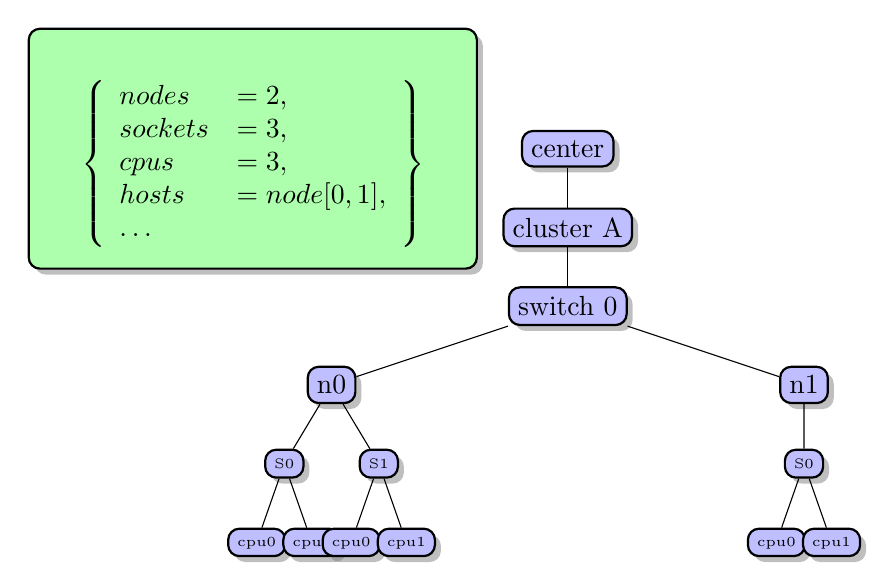
\begin{tikzpicture}[
    every node/.style = {drop shadow, rectangle, rounded corners,
        fill=blue!25, draw, thick},
    level 1/.style = {sibling distance = 6cm},
    level 3/.style = {sibling distance = 6cm},
    level 4/.style = {sibling distance = 12mm, font=\tiny},
    level 5/.style = {sibling distance = 7mm, font=\tiny, circle},
    level distance = 10mm,
    text depth = 0pt
   ]
    \node (center) {center}
      child {node (clusterA) {cluster A}
        child {node (switch0) {switch 0}
          child {node (n0) {n0}
            child {node (n0S0) {S0}
              child {node (n0S0cpu0) {cpu0}}
              child {node (n0S0cpu1) {cpu1}}
            }
            child {node (n0S1) {S1}
              child {node (n0S1cpu0) {cpu0}}
              child {node (n0S1cpu1) {cpu1}}
            }
          }
          child {node (n1) {n1}
            child {node (n1S0) {S0}
              child {node (n1S0cpu0) {cpu0}}
              child {node (n1S0cpu1) {cpu1}}
            }
        }
      }
    };%
%
%
 \visible<2->{%
   \node [fill=green!32] (summary) at (-4,0) {%
     \begin{minipage}[b][8em][c]{.45\textwidth}
     \[%
       \delimiterfactor=1000
       \left\{%
         \begin{array}{ll}
            nodes &= 2,   \\
            sockets &= 3, \\
            cpus &= 3,    \\
            hosts &= node[0,1], \\
            \ldots
         \end{array}
       \right\}%
     \]%
     \end{minipage}
   };%
 };%
 \end{tikzpicture}
 }%
\end{frame}

\begin{frame}{Plan}
\visible<+->
\centering Three target areas of research:
\begin{enumerate}
 \item<+-> Backend storage of resource configuration (Resource Inventory)
 \begin{itemize}
   \item<+-> Use CMB KVS for first version?
   \item<+-> Investigate available databases like MongoDB and Postgres
   \item<+-> Begin collecting ideas for RI API
 \end{itemize}
 \item<+-> Configuration syntax/language
 \begin{itemize}
   \item <+-> Experiemnt defining basic resources with Lua or YAML
 \end{itemize}
 \item<+-> Request syntax/language
 \begin{itemize}
   \item<+-> A discussion topic for the next meeting\ldots
 \end{itemize}
\end{enumerate}
\end{frame}

\end{document}
